\begin{frame}

	\frametitle{Spécifications fonctionnelles}
	\framesubtitle{Fonctionnalités globales}
	
	\only<1-2>
	{
		\begin{textblock*}{9cm}(2cm,2.5cm)
			{\LARGE Jeu d'arcade}
			\vfill
		\end{textblock*}
	}
	
	\only<1>
	{
		\begin{textblock*}{9cm}(2.7cm,3.75cm)
			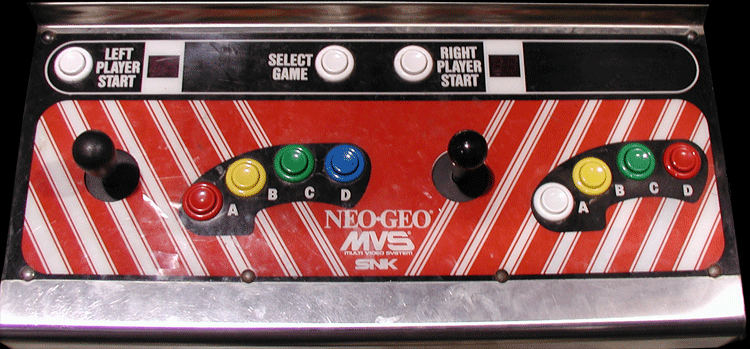
\includegraphics[width=9cm]{figures/panneau_de_controle_Neo_Geo_MVS_2p.png}
		\end{textblock*}
	}
	
	\only<1-2>
	{
		\invisible {invisible\\}
		\invisible {invisible\\}
		
		\begin{itemize}
			\setbeamertemplate{itemize item}[triangle]
			\item<2> Joystick 8 directions et 3 boutons
		\end{itemize}
		\begin{itemize}
			\setbeamertemplate{itemize item}[triangle]
			\item<2> Jouer 1P / 2P
		\end{itemize}
		\begin{itemize}
			\setbeamertemplate{itemize item}[triangle]
			\item<2> How to play
		\end{itemize}
		\begin{itemize}
			\setbeamertemplate{itemize item}[triangle]
			\item<2> Meilleurs scores
		\end{itemize}
	}
	
	\only<3->
	{
		\begin{textblock*}{8cm}(3.2cm,3cm)
			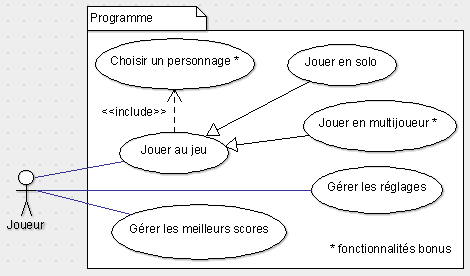
\includegraphics[width=8cm]{figures/use_case_metal_slug_general.png}
		\end{textblock*}
	}
	
\end{frame}
